% !TEX root = ../dg.tex

\section{Exterior Algebras and Differential Forms}

We just saw that 1-forms are $(0,1)$-tensor fields, but in general it's not quite natural to think of $k$-forms as tensor fields because we need to incorporate the alternating condition. We could do this by considering the subset of alternating tensor fields, but it turns out to be more natural to take a quotient of the tensor algebra to get something called the \emph{exterior algebra}.

Specifically, just as the tensor product is a way of turning multilinear maps into linear maps, the \emph{exterior product} will turn out to be the way to turn alternating multilinear maps into linear maps. Even though we haven't actually defined the exterior product yet, it might seem silly to introduce another new product; after all, alternating multilinear maps are multilinear so the tensor product \emph{already} turns them into linear maps.

That being the case, the exterior product does this in much lower dimension, so it's still worthwhile. At the most extreme level, you can see this because the natural space in which the tensor product lives (as a binary operation) is the tensor algebra $\mathcal{T}(V)$ (or, if you like, only the $(r,0)$ part $V_0^0 \otimes V_1^0 \otimes V_2^0 \otimes \dots$), which is always infinite-dimensional. Whereas the exterior product will be a binary operation on the exterior algebra, which will turn out to be finite-dimensional if $V$ is. And, if you weren't already aware, finite-dimensional vector spaces are \emph{much, much nicer} than infinite-dimensional vector spaces: it's always worthwhile to make the effort to work in finite dimensions if at all possible.

\begin{definition}\label{def:exterior algebra}
	Let $\mathcal{C}(V) = \bigoplus_{k \geq 0} V_k^0$ be the algebra of $(\cdot , 0)$ tensors on a vector space $V$ and let $\mathcal{I}(V)$ be the two-sided ideal generated by elements of the form $v \otimes v$ for $v \in V$. Then the \emph{exterior algebra} of $V$ is the quotient
	\[
		\ext{}(V) := \mathcal{C}(V)/\mathcal{I}(V).
	\]
	This is a graded algebra with product denoted by $\wedge$, which is just the product induced by $\otimes$: the residue class of $v_1 \otimes v_2 \otimes \dots \otimes v_k$ is denoted $v_1 \wedge v_2 \wedge \dots \wedge v_k$.
\end{definition}

The grading is given by the degree of the wedge product, since
\[
	\ext{}(V) = \bigoplus_{k \geq 0} \ext{k}(V),
\]
where $\ext{k}(V) = V_k^0/\mathcal{I}_k$, and $\mathcal{I}_k = \mathcal{I}(V) \cap V_k^0$.

\begin{proposition}\label{prop:wedge product graded commutative}
	If $a \in \ext{k}(V)$ and $b \in \ext{\ell}(V)$, then $b \wedge a = (-1)^{k\ell} a \wedge b$.
\end{proposition}

\begin{exercise}
	Prove \Cref{prop:wedge product graded commutative}.
\end{exercise}

\begin{corollary}\label{cor:wedge product alternating}
	$v_{\sigma(1)} \wedge \dots \wedge v_{\sigma(k)} = \sgn(\sigma) v_1 \wedge \dots \wedge v_k$ for any permutation $\sigma$ of $\{1,\dots, k\}$.
\end{corollary}

In particular, this says that we can always rearrange any wedge product to have the terms in any order we like. For example, if the terms are indexed (e.g., if they come from some ordered basis), we can always make the indices appear in increasing order at the cost of a sign.

\begin{proposition}\label{prop:exterior power basis}
	If $\{e_1, \dots, e_n\}$ is a basis for $V$, then 
	\[
		\{e_{i_1} \wedge \dots \wedge e_{i_k} : 1 \leq i_1 < i_2 < \dots < i_k \leq n\}
	\]
	is a basis for $\ext{k}(V)$. In particular,
	\[
		\dim \ext{k}(V) = \begin{cases} \binom{n}{k} & \text{if } 0 \leq k \leq n \\ 0 & \text{else.}\end{cases}
	\]
	Hence,
	\[
		\dim \ext{}(V) = \sum_{k \geq 0} \dim \ext{k}(V) = \sum_{k=0}^n \binom{n}{k} = 2^n.
	\]	
\end{proposition}

\begin{exercise}
	Prove \Cref{prop:exterior power basis}.
\end{exercise}

This is exactly the finite-dimensionality described above. Even if we're just interested in alternating, bilinear maps $V \times V \to W$, $\dim \ext{2}(V) = \binom{n}{2}$ is less than half of $\dim V^{\otimes 2} = n^2$, so working with the exterior power rather than the tensor power means we're doing linear algebra in half the dimensions, which is almost always worthwhile computationally.

As you would expect, the exterior products satisfy a universal property analogous to the one satisfied by tensor products:

\begin{theorem}[Universal Property of the Exterior Product]\label{thm:exterior product universal property}
	If $\phi\from V^k \to \ext{k}(V)$ is the map given by $(v_1, \dots , v_k) \mapsto v_1 \wedge \dots \wedge v_k$ and $F \from V^k \to W$ is an alternating multilinear map, then there exists a unique linear map $\widetilde{F} \from \ext{k}(V) \to W$ making the following diagram commute:
	\ifplastex
		\begin{center}
			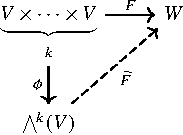
\includegraphics[height=1.5in]{cd4}
		\end{center}
	\else	
		\[
			\begin{tikzcd}
				\underbrace{V \times \dots \times V}_k \arrow[r,"F"] \arrow[d,"\phi"'] & W \\
				\ext{k}(V) \arrow[ur,"\widetilde{F}"',dashed]
			\end{tikzcd}
		\]
	\fi
	Again, this uniquely characterizes $\ext{k}(V)$ up to isomorphism.
\end{theorem}

\begin{example}
	Suppose $V = \R^n$, and suppose $F \from \R^n \to \R$ is alternating and multilinear. We know that this factors through a linear map $\ext{n}(\R^n) \to \R$; since $\dim \ext{n}\R^n = \binom{n}{n} = 1$, we know that $\ext{n}\R^n \cong \R$, and so (once we've chosen a basis for $\ext{n}\R^n$, which witnesses the isomorphism $\ext{n}\R^n \cong \R$), $\widetilde{F}$ has to be of the form $x \mapsto ax$ for some scalar $a$. We can already see that this is going to imply that $F$ is unique up to the choice of the scalar $a$.
	
	Let's work out what $\phi \from (\R^n)^n \to \ext{n}\R^n$ is. Let $e_1, \dots , e_n$ be the standard basis for $\R^n$, so that each $v_i = \sum_{j_i=1}^n a_{ij_i} e_{j_i}$. Then repeatedly applying \Cref{cor:wedge product alternating} and the alternating property of the wedge product yields
	\begin{align*}
		\phi(v_1, \dots , v_n) & = \phi\left(\sum_{j_1=1}^n a_{1j_1}e_{j_1}, \dots , \sum_{j_n=1}^n a_{nj_n}e_{j_n}\right)  \\
		& = \left(\sum_{j_1=1}^n a_{1j_1}e_{j_1}\right) \wedge \dots \wedge \left(\sum_{j_n=1}^n a_{nj_n} e_{j_n}\right) \\
		& = \sum_{j_1=1}^n \dots \sum_{j_n=1}^n a_{1j_1} \cdots a_{n j_n} e_{j_1} \wedge \dots \wedge e_{j_n} \\
		& = \sum_{\sigma \in S_n} \left[ \left(\prod_{i=1}^n a_{i \sigma(i)}\right) e_{\sigma(1)} \wedge \dots \wedge e_{\sigma(n)}\right]  \\
		& = \sum_{\sigma \in S_n} \left[ \sgn(\sigma) \left(\prod_{i=1}^n a_{i\sigma(i)}\right) e_1 \wedge \dots \wedge e_n \right] \\
		& = \left[ \sum_{\sigma \in S_n} \sgn(\sigma) \left(\prod_{i=1}^n a_{i\sigma(i)}\right)\right] e_1 \wedge \dots \wedge e_n  \\
		& = \det \begin{bmatrix} v_1 & \cdots & v_n \end{bmatrix} e_1 \wedge \dots \wedge e_n,
	\end{align*}
	where we just recognized the Leibniz formula for the determinant in the last equality.
	
	Since $\{e_1 \wedge \dots \wedge e_n\}$ is our preferred basis for $\ext{n}\R^n$, inducing the isomorphism $\R \overset{\cong}{\to} \ext{n}\R^n$ given by $1 \mapsto e_1 \wedge \dots \wedge e_n$, we see that
	\[
		F(v_1, \dots , v_n) = (\widetilde{F} \circ \phi)(v_1, \dots , v_n) = \widetilde{F}(\phi(v_1, \dots , v_n)) = \widetilde{F}(\det \begin{bmatrix} v_1 & \cdots & v_n \end{bmatrix} e_1 \wedge \dots \wedge e_n) = a \det \begin{bmatrix} v_1 & \cdots & v_n \end{bmatrix}
	\]
	for some $a \in \R$, which (re)proves \Cref{thm:determinant}, which says that the determinant is, up to scale, the unique alternating multilinear map $(\R^n)^n \to \R$.
\end{example}

If we let $W = \R$ (or whatever the base field is) in \Cref{thm:exterior product universal property}, then we see that alternating multilinear functionals on $V^k$ correspond precisely to linear functionals on $\ext{k}V$; that is, to elements of the dual space $\left(\ext{k}V\right)^\ast$. But of course this is essentially how we ``defined'' differential $k$-forms in \Cref{def:informal differential form}: at each point a $k$-form should exactly be an alternating multilinear functional on the product of $k$ copies of the tangent space at that point.

\begin{definition}\label{def:differential form}
	The \emph{exterior $k$-bundle} on a manifold $M$ is
	\[
		\ext{k}(M) := \bigsqcup_{p \in M} \ext{k}\left(\left(T_pM\right)^\ast\right)
	\]
	and the \emph{exterior algebra bundle} over $M$ is
	\[
		\ext{} (M) := \bigsqcup_{p \in M} \ext{} \left(\left(T_pM\right)^\ast\right).
	\]
	Both of these are smooth manifolds.
	
	A \emph{differential $k$-form} on $M$ is a smooth section of $\ext{k}(M)$; that is, a smooth map $\omega\from M \to \ext{k}(M)$ so that $\omega(p) \in \ext{k}\left(\left(T_pM\right)^\ast\right)$. The space of $k$-forms on $M$ is denoted $\Omega^k(M)$, and we let $\Omega^\ast(M) := \displaystyle \bigoplus_{k=0}^n \Omega^k(M)$, which is the algebra of differential forms on $M$.
\end{definition}

If you've been reading very closely, you might have noticed that I played fast and loose with parentheses and stars above. The discussion in the paragraph before \Cref{def:differential form} suggests that, if $\omega$ is a $k$-form (that is, an alternating, multilinear map $\mathfrak{X}(M)^k \to C^\infty(M)$ according to our informal definition), then at a point $p \in M$ we should expect that $\omega(p) \in \left(\ext{k}\left(T_pM\right)\right)^\ast$. But I've just defined $\omega(p)$ as an element of $\ext{k}\left(\left(T_pM\right)^\ast \right)$! So what's going on?

First of all, $\ext{k}\left(\left(T_pM\right)^\ast \right)$ is (at least to me) conceptually nicer than $\left(\ext{k}\left(T_pM\right)\right)^\ast$: it's an exterior power itself, rather than being the dual of an exterior power, and so it obviously fits into an exterior algebra, namely $\ext{}\left(\left(T_pM\right)^\ast\right)$. So that's the reason for wanting to define exterior bundles in terms of $\ext{k}\left(\left(T_pM\right)^\ast\right)$ rather than $\left(\ext{k}\left(T_pM\right)\right)^\ast$.

Of course, the reason I can do this is because they're isomorphic:

\begin{lemma}\label{lem:exterior powers and duals}
	Suppose $V$ is a finite-dimensional vector space. Then
	\[
		\ext{k}(V^\ast) \cong \left(\ext{k} V\right)^\ast,
	\]
	and therefore
	\[
		\ext{}(V^\ast) \cong \left(\ext{}(V)\right)^\ast.
	\]
\end{lemma}

The strategy here is to find a nondegenerate pairing between $\ext{k}(V^\ast)$ and $\ext{k} (V)$. Recall that a \emph{nondegenerate pairing} of vector space $V$ and $W$ is a bilinear map
\[
	(\cdot , \cdot ) \from V \times W \to \R
\]
with the property that, for any nonzero $w \in W$, there exists $v \in V$ so that $(v,w) \neq 0$ (and similarly when you swap the roles of $v$ and $w$). Notice, in particular, that a pairing corresponds uniquely to a linear map $V \otimes W \to \R$; that is, an element of $(V \otimes W)^\ast$.

If there is a nondegenerate pairing of $V$ and $W$, then it induces injective maps $\phi \from V \to W^\ast$ and $\psi \from W \to V^\ast$ given by
\[
	\phi(v)(w) := (v,w) =: \psi(w)(v).
\]

\begin{example}
	An inner product $\langle \cdot , \cdot \rangle$ on $V$ is a nondegenerate pairing of $V$ with itself: after all, if $v \neq 0$, then $\langle v , v \rangle \neq 0$ by the positivity of the inner product. Hence, the inner product induces an injective map $V \to V^\ast$ which turns out to be an isomorphism if $V$ is finite-dimensional (or more generally if we take $V^\ast$ to be the continuous dual space rather than the algebraic dual space); this isomorphism is the content of the Riesz representation theorem.
\end{example}

In finite dimensions, we know that $V \cong V^\ast$ and $W \cong W^\ast$, so the composition $V \overset{\phi}{\hookrightarrow} W^\ast \cong W \overset{\psi}{\hookrightarrow} V^\ast$ gives an injective (and therefore also surjective) map $V \to V^\ast$, which implies that $\phi$ and $\psi$ had to be bijective, and therefore isomorphisms. In particular, this implies that $V \cong W^\ast$ (and therefore also $W \cong V^\ast$ and indeed $V \cong W$).

So the strategy for proving \Cref{lem:exterior powers and duals} is to find a nondegenerate pairing of $\ext{k}(V^\ast)$ and $\ext{k}(V)$, which will imply the result.\footnote{At a more basic level, it's not hard to see that these vector spaces have the same dimension, and hence must be abstractly isomorphic, but it's helpful to make this isomorphism more concrete with the pairing.}

\begin{proof}[Proof of \Cref{lem:exterior powers and duals}]
	To find the pairing $(\cdot , \cdot ) \from \ext{k}(V^\ast) \times \ext{k} (V) \to \R$, suppose first that $\alpha \in \ext{k}(V^\ast)$ and $b \in \ext{k}(V)$ are \emph{decomposable}, meaning that $\alpha = \alpha_1 \wedge \dots \wedge \alpha_k$ for $\alpha_1 , \dots , \alpha_k \in V^\ast$ and $b = b_1 \wedge \dots \wedge b_k$ for $b_1, \dots , b_k \in V$. Then define
	\begin{equation}\label{eq:pairing}
		(\alpha, b) := \det \left( \begin{bmatrix} \alpha_i(b_j) \end{bmatrix}_{i,j}\right).
	\end{equation}
	Since arbitrary elements of $\ext{k}(V^\ast)$ and $\ext{k}(V)$ are linear combinations of decomposable elements, we define $(\cdot , \cdot ) \from \ext{k}(V^\ast) \times \ext{k} (V) \to \R$ by extending the above linearly. 
	
	It is straightforward (but somewhat tedious) to check that $(\cdot , \cdot)$ is nondegenerate, and thus induces the desired isomorphism $\ext{k}(V^\ast) \overset{\cong}{\to} \left(\ext{k}(V)\right)^\ast$. Doing this for each $k$ shows that the exterior algebra
	\[
		\ext{}(V^\ast) = \bigoplus_{k=0}^{\dim V} \ext{k}(V^\ast) \cong \bigoplus_{k=0}^{\dim V} \left(\ext{k}(V)\right)^\ast \cong \left( \bigoplus_{k=0}^{\dim V} \ext{k}(V)\right)^\ast = \left(\ext{}(V)\right)^\ast.
	\]
\end{proof}

Notice that this argument---and especially \eqref{eq:pairing}---really validates the idea that all alternating multilinear maps are, in some sense, determinants. 

\subsection{Differential Forms in Local Coordinates}
\label{sub:differential_forms_in_local_coordinates}

\Cref{def:differential form} is not the easiest thing to compute with, so let's try to understand what differential forms look like in local coordinates. Suppose $M$ is an $n$-manifold, $\omega \in \Omega^k(M)$ is a $k$-form, and $p \in M$. Let $(U,\phi)$ be a local coordinate chart in a neighborhood of $p$, and define the functions $x_i \from \phi(U) \to \R$ by $x_i(\phi(a_1, \dots , a_n)) = a_i$. In other words, the function $x_i$ reports the $i$th local coordinate of a point in this coordinate chart.

Now, each function $x_i$ has a differential $dx_i$ which (as in \Cref{ex:differentials as 1-forms}) is a 1-form on $\phi(U) \subset M$. In particular, at $p$ the differential $(dx_i)_p \from T_p M \to T_{x_i(p)}\R \cong \R$ is a linear functional on $T_pM$; that is, an element of the dual space $\left(T_pM\right)^\ast$.

If $\left\{\frac{\partial}{\partial x_1}, \dots , \frac{\partial}{\partial x_n}\right\}$ is the local coordinate basis for $T_pM$ associated to our chart, I claim that $\{(dx_1)_p, \dots , (dx_n)_p\}$ gives the corresponding dual basis for $\left(T_pM\right)^\ast$: by \Cref{lem:vector fields and differentials},
\[
	(dx_i)_p \left(\frac{\partial}{\partial x_j}\right) = \frac{\partial}{\partial x_j}(x_i) = \delta_{ij}.
\]

In what follows I'm going to drop the subscript $p$ and just say $\{dx_1, \dots, dx_n\}$ is a basis for $\left(T_pM\right)^\ast = \ext{1}\left(\left(T_pM\right)^\ast\right)$. More generally, as in \Cref{prop:exterior power basis}, $\{dx_{i_1} \wedge \dots \wedge dx_{i_k}: 1 \leq i_1 < \dots < i_k \leq n\}$ gives a basis for $\ext{k}\left(\left(T_pM\right)^\ast \right)$, and hence at the point $p$ our $k$-form $\omega$ can be written as
\[
	\omega_p = \sum_I a_I dx_I,
\]
where $I = (i_1, \dots , i_k)$ is any $k$-tuple of distinct, sorted indices and $dx_I$ is shorthand for $dx_{i_1} \wedge \dots \wedge dx_{i_k}$.

\begin{example}
	On $\R^2$ we have global coordinates, so every $\omega \in \Omega^1(\R^2)$ is of the form $\omega = f\, dx + g\, dy$ for smooth functions $f,g \in C^\infty (\R^2)$. So if $\omega = f\, dx + g \, dy$ and $\eta = h\, dx + m\, dy$ are two 1-forms, we will have
	\[
		\omega \wedge \eta = (f\, dx + g\, dy) \wedge (h\, dx + m\, dy) = (fm - gh) dx \wedge dy.
	\]
	In particular,
	\[
		(\omega \wedge \eta)(U,V) = (\omega \wedge \eta)\left(u_1 \frac{\partial}{\partial x} + u_2 \frac{\partial}{\partial y}, v_1 \frac{\partial}{\partial x} + v_2 \frac{\partial}{\partial y}\right) = (fm-gh)(u_1 v_2 - u_2 v_1).
	\]
\end{example}

\begin{example}
	On $\R^3$, if $\omega, \eta \in \Omega^1(\R^3)$ with $\omega = f \, dx + g \, dy + h \, dz$ and $\eta = a\, dx + b\, dy + c \, dz$, then
	\[
		\omega \wedge \eta = (gc-hb)dy \wedge dz + (ha-fc)dz \wedge dx + (fb-ga)dx \wedge dy.
	\]
	Compare with the cross product
	\[
		\omega^\sharp \times \eta^\sharp = \left(f \frac{\partial}{\partial x} + g \frac{\partial}{\partial y}+h \frac{\partial}{\partial z}\right) \times \left( a \frac{\partial}{\partial x} + b \frac{\partial}{\partial y}+ c \frac{\partial}{\partial z}\right) = (gc-hb) \frac{\partial}{\partial x} + (ha-fc) \frac{\partial}{\partial y} + (fb-ga) \frac{\partial}{\partial z}.
	\]
	
	Also, if $\mu = p\, dy \wedge dz + q\, dz \wedge dx + r\, dx \wedge dy$, then
	\[
		\omega \wedge \mu = (f \, dx + g \, dy + h \, dz ) \wedge (p\, dy \wedge dz + q\, dz \wedge dx + r\, dx \wedge dy) = (fp + gq + hr) dx \wedge dy \wedge dz.
	\]
	Compare with the dot product
	\[
		\omega^\sharp \cdot (\star \mu)^\sharp = \left(f \frac{\partial}{\partial x} + g \frac{\partial}{\partial y}+h \frac{\partial}{\partial z}\right) \times \left( p \frac{\partial}{\partial x} + q \frac{\partial}{\partial y}+ r \frac{\partial}{\partial z}\right) = fp + gq + hr.
	\]
\end{example}

Locally, any manifold looks like $\R^n$, so these computations work just as well in local coordinates on 2- and 3-manifolds.